\chapter{Speech Programming}
\label{speech-chapter}

\section{Introduction}

Little Sound Dj contains fifty-nine discrete speech sounds (called allophones), stored in the first four kit banks. By combining these sounds, it is possible to create any English word or phrase.

\section{Linguistics}

A few basic linguistic concepts will help you create your own library of words. First, there is no one-to-one correspondence between written letters and speech sounds; secondly, speech sounds are acoustically different depending on their position within a word.

The first problem compares to the problem that a child encounters when it learns to read. Each sound in a language may be represented by more than one letter, and conversely, each letter may represent more than one sound. Because of these spelling irregularities, it is necessary to think in terms of sounds, not letters, when using allophones.

The second, and equally important, point to understand is that the acoustic signal of a speech sound may differ depending on its position within a word. For example, the initial K sound in coop will be acoustically different from the K's in keep and speak.

\section{Programming Words}

Little Sound Dj has a special speech instrument. It is locked to instrument number \$40 and can be used in the wave channel. It contains a set of 42 words, mapped out from note C-3 to note F-6. 

\begin{figure}[htpb]
	\begin{center}
	\fbox{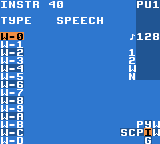
\includegraphics{speech}}
	\end{center}
	\caption{Speech Instrument Screen}
	\label{fig:speech}
\end{figure}
\begin{figure}[htpb]
	\begin{center}
	\fbox{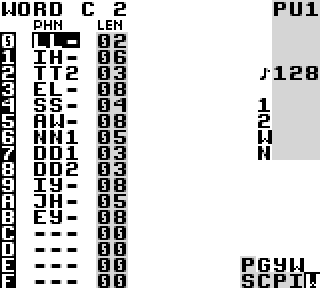
\includegraphics{word}}
	\end{center}
	\caption{Example Word}
	\label{fig:word}
\end{figure}

		If you want to edit a word, press \textsc{select+right} to get to the word screen. It has two columns; the left column contains the allophones to be played, the right column sets duration. The word in figure~\ref{fig:word} is programmed to say "Little Sound Dj."

		In order to make things easy to remember, it is possible to rename the words by tapping A in the speech instrument screen. If you want to, it is also possible to cut and paste words in the speech instrument screen.

\section{Guidelines for Using the Allophones}

Allophones marked with * loop indefinitely. 

\subsection{Short vowels}

\begin{description}
\item[*IH] sitting, stranded
\item[*EH] extent, gentlemen
\item[*AE] extract, acting
\item[*UH] cookie, full
\item[*AD] talking, song
\item[*AX] lapel, instruct
\end{description}

\subsection{Long vowels}

\begin{description}
\item[IY] treat, people, penny
\item[EY] great, statement, tray
\item[AY] kite, sky, mighty
\item[OI] noise, toy, voice
\item[UW1] after clusters with YY: computer
\item[UW2] in monosyllabic words: two, food
\item[OW] zone, close, snow
\item[AW] sound, mouse, down
\item[EL] little, angle, gentlemen
\end{description}

\subsection{R-colored vowels}

\begin{description}
\item[ER1] letter, furniture, interrupt
\item[ER2] monosyllables: bird, fern, burn
\item[OR] fortune, adorn, store
\item[AR] farm, alarm, garment
\item[YR] hear, earring, irresponsible
\item[XR] hair, declare, stare
\end{description}

\subsection{Resonants}
\begin{description}
\item[WW] we, warrant, linguist
\item[RR1] initial position: read, write, x-ray
\item[RR2] initial clusters: brown, crane, grease
\item[LL] like, hello, steel
\item[YY1] clusters: cute, beauty, computer
\item[YY2] initial position: yes, yarn, yo-yo
\end{description}

\subsection{Voiced fricatives}
\begin{description}
\item[VV] vest, prove, even
\item[DH1] word-initial position: this, then, they
\item[DH2] word-final and between vowels: bathe, bathing
\item[ZZ] zoo, phase
\item[ZH] beige, pleasure
\end{description}

\subsection{Voiceless fricatives}
\begin{description}
\item[*FF] fire, fox
\item[*TH] this, they
\item[*SS] sit, smile
\item[SH] shirt, leash, nation
\item[HH1] before front vowels: YR, IY, IH, EY, EH, XR, AE
\item[HH2] before back vowels: UW, UH, OW, OY, AO, OR, AR
\item[WH] white, whim, twenty
\end{description}

\subsection{Voiced stops}
\begin{description}
\item[BB1] final position: rib; between vowels: fibber, in clusters: bleed, brown
\item[BB2] initial position before a vowel: beast
\item[DD1] final position: played, end
\item[DD2] initial position: down; clusters: drain
\item[GG1] before high front vowels: YR, IY, IH, EY, EH, XR
\item[GG2] before high back vowels: UW, UH, OW, OY, AX; and clusters: green, glue
\item[GG3] before low vowels: AE, AW, AY, AR, AA, AO, OR, ER; and medial clusters: anger; and final position: peg
\end{description}

 
\subsection{Voiceless stops}
\begin{description}
\item[PP] pleasure, ample, trip
\item[TT1] final clusters before SS: tests, its
\item[TT2] all other positions: test, street
\item[KK1] before front vowels: YR, IY, IH, EY, EH, XR, AY, AE, ER, AX; initial clusters: cute, clown, scream
\item[KK2] final position: speak; final clusters: task
\item[KK3] before back vowels: UW, UH, OW, OY, OR, AR, AO; initial clusters: crane, quick, clown, scream
\end{description}

\subsection{Affricates}
\begin{description}
\item[CH] church, feature
\item[JH] judge, injure
\end{description}

\subsection{Nasal}
\begin{description}
\item[MM] milk, alarm, example
\item[NN1] before front and central vowels: YR, IY, IH, EY, EH, XR, AE, ER, AX, AW, AY, UW; final clusters: earn
\item[NN2] before back vowels: UH, OW, OY, OR, AR, AA
\end{description}



